\documentclass[tikz,border=6pt]{standalone}
% Shared visual language for the book's standalone vector figures.
% Keep this file compatible with the TeX Live version used by LyX.
\usepackage{amsmath,amssymb}
\usepackage{array,booktabs}
\usepackage{pgfplots}
\usepackage{pgfplotstable}
\usetikzlibrary{arrows.meta,calc,positioning}
\pgfplotsset{compat=1.17}

\definecolor{BookBlue}{HTML}{0072B2}
\definecolor{BookOrange}{HTML}{D55E00}
\definecolor{BookGreen}{HTML}{009E73}
\definecolor{BookGray}{HTML}{666666}
\definecolor{BookLightGray}{HTML}{D9D9D9}

\pgfplotsset{
  book axis/.style={
    axis line style={black!75,line width=0.55pt},
    tick style={black!75,line width=0.45pt},
    tick label style={font=\small},
    label style={font=\small},
    legend style={
      font=\small,
      draw=none,
      fill=none,
      cells={anchor=west},
    },
    grid style={BookLightGray,line width=0.35pt},
    major grid style={BookLightGray,line width=0.35pt},
  },
}

\begin{document}
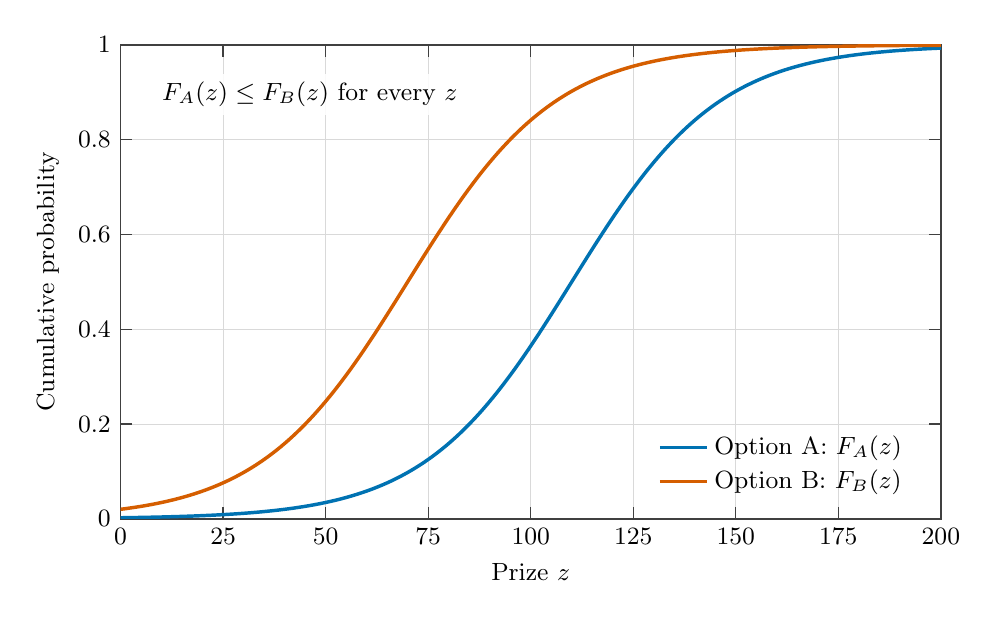
\begin{tikzpicture}
  \begin{axis}[
    book axis,
    width=12.0cm,
    height=7.6cm,
    xmin=0,xmax=200,
    ymin=0,ymax=1,
    xtick={0,25,...,200},
    ytick={0,0.2,...,1},
    xlabel={Prize $z$},
    ylabel={Cumulative probability},
    grid=major,
    legend pos=south east,
  ]
    \addplot[BookBlue,line width=1.25pt,domain=0:200,samples=201]
      {1/(1+exp(-(x-110)/18))};
    \addlegendentry{Option A: $F_A(z)$}
    \addplot[BookOrange,line width=1.25pt,domain=0:200,samples=201]
      {1/(1+exp(-(x-70)/18))};
    \addlegendentry{Option B: $F_B(z)$}
    \node[
      anchor=north west,
      fill=white,
      fill opacity=0.88,
      text opacity=1,
      inner sep=3pt,
      font=\small,
    ] at (axis cs:8,0.94) {$F_A(z)\leq F_B(z)$ for every $z$};
  \end{axis}
\end{tikzpicture}
\end{document}
